\documentclass[a4paper]{article}

\usepackage[T1]{fontenc}
\usepackage{graphicx}
\usepackage{amsmath}
\usepackage[utf8]{inputenc}
\usepackage{enumitem}
\setlist[description]{style=unboxed}

\usepackage{tikz}
\usepackage{pgfplots}
\usepackage{circuitikz}

\usetikzlibrary{calc,positioning,shapes,decorations.pathreplacing}

\tikzset{
	short/.style={draw,rectangle,text height=3pt,text depth=13pt,
		text width=7pt,align=center,fill=gray!30},
	long/.style={short,text width=1.5cm},
	verylong/.style={short,text width=4.5cm}
}

\begin{document}
\section{AC voltage rectifier and regulator}

\subsection{Introduction}

For fully functional operation, submarine/robot arm/habitat is equipped with 
lot of computer based subsystems and electronic devices which operate on DC 
voltage. To ensure proper operation the DC voltage has to be stable and without 
noise.

To ensure stable DC voltage, linear regulator on Fig. 1. is used. Due to 
extreme conditions in the system, regulators often fail and components have to 
be repaired or replaced with proper spare part.

In this task, your job is to:
\begin{itemize}
\item identify components that failed in different scenarios, 
\item find the proper replacement parts, 
\item ensure that the output voltage ripple is within the boundaries with proper low pass filter,
\item find the probability of future malfunction in standby redundant system.
\end{itemize}



\begin{figure}[h!]
\centering
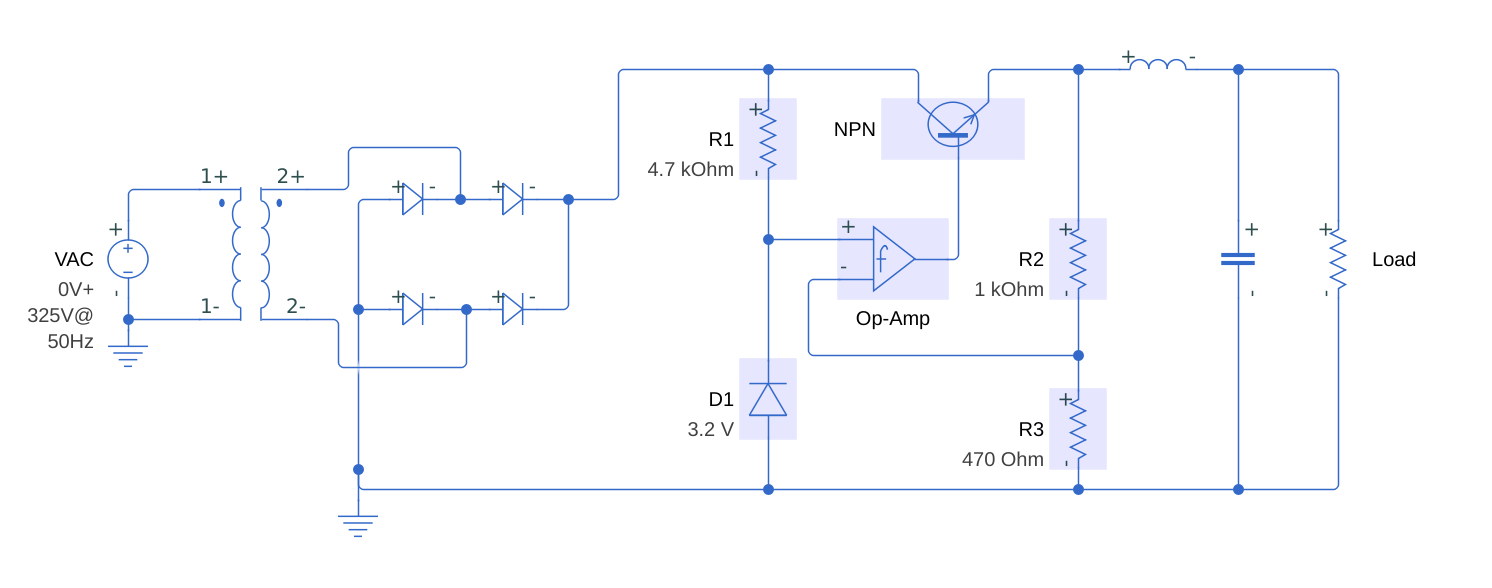
\includegraphics[width=\linewidth]{images/reg.png}

\caption{Rectifier and linear regulator.}
\end{figure}

\subsection{Identifying failed components}

\textbf{1. failure scenario - Zener diode}

\textbf{2. failure scenario - Diode in rectifier bridge}

\textbf{3. failure scenario - Resistor}




\end{document}